\documentclass{beamer}
\usepackage[utf8]{inputenc}

\usetheme{Madrid}
\usecolortheme{default}
\usepackage{amsmath,amssymb,amsfonts,amsthm}
\usepackage{txfonts}
\usepackage{tkz-euclide}
\usepackage{listings}
\usepackage{adjustbox}
\usepackage{array}
\usepackage{tabularx}
\usepackage{gvv}
\usepackage{lmodern}
\usepackage{tikz}
\usepackage{graphicx}

\setbeamertemplate{page number in head/foot}[totalframenumber]

\lstset{
    language=C,
    basicstyle=\ttfamily\small,
    keywordstyle=\color{blue},
    stringstyle=\color{orange},
    commentstyle=\color{green!60!black},
    numbers=left,
    numberstyle=\tiny\color{gray},
    breaklines=true,
    showstringspaces=false,
}

%------------------------------------------------------------
\title{5.2.9}
\date{oct 10, 2025}
\author{ADUDOTLA SRIVIDYA - EE25BTECH11006}

\begin{document}

\frame{\titlepage}
\begin{frame}{Question}
Solve the simultaneous linear equations
$5u-4v+8=0$ , $7u+6v-9=0$.
\end{frame}

\begin{frame}{Solution}
    \begin{align}
5u - 4v &= -8 
\end{align}
\begin{align}
7u + 6v &= 9
\end{align}

\begin{align}
\myvec{5 & -4 \\ 7 & 6}\myvec{u \\ v}=\myvec{-8 \\ 9}
\end{align}

Augmented matrix,
\begin{align}
\myvec{5 & -4 & -8 \\ 7 & 6 & 9} 
\end{align}
\end{frame}

\begin{frame}{Solution}
    \begin{align}
\myvec{5 & -4 & -8 \\ 7 & 6 & 9}
\xrightarrow{R_2 \rightarrow 5R_2-7R_1}
\myvec{5 & -4 & -8 \\ 0 & 58 & 101}
\xrightarrow{R_2 \rightarrow \dfrac{r_2}{58}}
\myvec{5 & -4 & -8 \\ 0 & 1 & \dfrac{101}{58}}
\end{align}
\begin{align}
\myvec{5 & -4 & -8 \\ 0 & 1 & \dfrac{101}{58}}
\xrightarrow{R_1 \rightarrow R_1+4R_2}
\myvec{5 & 0 & -\dfrac{30}{29} \\ 0 & 1 & \dfrac{101}{58}}
\xrightarrow{R_1 \rightarrow \dfrac{R_1}{5}}
\myvec{1 & 0 & -\dfrac{6}{29} \\ 0 & 1 & \dfrac{101}{58}}
\end{align}
\end{frame}

\begin{frame}{Solution}
    Thus, the solution vector is
\begin{align}
    \myvec{u \\ v}=\myvec{-\dfrac{6}{29} \\ \dfrac{101}{58}}
\end{align}
\end{frame}

\begin{frame}[fragile]
\frametitle{Python,C,Python+C codes}
codes permalink
\end{frame}

\begin{frame}{plot}
    \begin{figure}
    \centering
    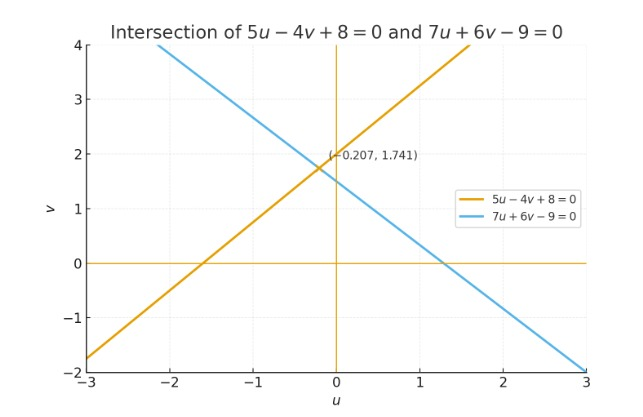
\includegraphics[width=0.5\columnwidth]{figs/fig.jpeg}
    \caption{fig}
    \label{fig:}
\end{figure}
\end{frame}

\end{document}